% !TeX program = pdflatex
% Quantum-targeted manuscript: A Resource Theory of Shared Complex Structure.
%
% Compile with: latexmk -pdf main.tex   (or: pdflatex; bibtex; pdflatex x2)
%
% The quantumarticle class is the Quantum journal style.

\documentclass[a4paper,onecolumn,noarxiv]{quantumarticle}
\pdfoutput=1

\usepackage[utf8]{inputenc}
\usepackage[T1]{fontenc}
\usepackage{amsmath, amssymb, amsthm, mathtools}
\usepackage{graphicx}
\usepackage[colorlinks=true,linkcolor=blue,citecolor=blue,urlcolor=blue]{hyperref}
\usepackage{booktabs}
\usepackage{microtype}
\usepackage{tikz}
\usetikzlibrary{arrows.meta, positioning, fit, backgrounds, shapes.geometric}

% Theorem environments
\theoremstyle{plain}
\newtheorem{theorem}{Theorem}
\newtheorem{proposition}[theorem]{Proposition}
\newtheorem{corollary}[theorem]{Corollary}
\newtheorem{lemma}[theorem]{Lemma}

\theoremstyle{definition}
\newtheorem{definition}[theorem]{Definition}
\newtheorem{example}[theorem]{Example}

\theoremstyle{remark}
\newtheorem*{remark}{Remark}

% Macros
\newcommand{\R}{\mathbb{R}}
\newcommand{\C}{\mathbb{C}}
\newcommand{\HC}{H_{\C}}
\newcommand{\HR}{H_{\R}}
\newcommand{\KAB}{K_{AB}}
\newcommand{\Pplus}{P_{+}}
\newcommand{\Pminus}{P_{-}}
\newcommand{\Hplus}{H_{+}}
\newcommand{\Hminus}{H_{-}}
\newcommand{\Aop}{\mathsf{A}}
\newcommand{\Bop}{\mathsf{B}}
\newcommand{\Mop}{M}
\newcommand{\JAB}{J_{AB}}
\newcommand{\FAB}{\mathcal{F}_{AB}}
\newcommand{\Tr}{\operatorname{Tr}}
\newcommand{\Phid}{\Phi^{\dagger}}
\newcommand{\Ldag}{\mathcal{L}^{\dagger}}
\newcommand{\Lleak}{L}
\newcommand{\sameI}{same-$i$}

\title{A Resource Theory of Shared Complex Structure in Real Quantum Composition}

\author{Julian Juan%
  \thanks{Correspondence: \href{mailto:bubgaming3@gmail.com}{bubgaming3@gmail.com}. ORCID: \href{https://orcid.org/XXXX-XXXX-XXXX-XXXX}{XXXX-XXXX-XXXX-XXXX}.}}
\affiliation{Independent researcher}

\date{May 16, 2026}

\begin{document}

\maketitle

\begin{abstract}
Whether real Hilbert spaces can support quantum theory is a question that lives in
composition, not in individual systems. A single complex system admits a real
reformulation by replacing multiplication by $i$ with an orthogonal complex structure
$J$. When two such systems are combined, however, the full real tensor product is
strictly larger than the realification of the complex tensor product, and the extra
degrees of freedom encode disagreement between the two local complex structures. We
show that ordinary complex composition is exactly the zero-leakage, aligned-sector
subset of the full real tensor product. The ``alignment cost'' is captured by a single
basis-independent monotone --- the \textbf{same-$i$ leakage} $\Lleak(\rho) =
\Tr(\Pminus\rho)$ --- and we develop it into a complete resource theory.

Our main quantitative results are: (i) the coherent cross-sector amplitude is bounded
by $\|\Pplus\rho\Pminus\|_1 \le \sqrt{\Lleak(1-\Lleak)}$, saturated by pure coherent
cross-sector states; (ii) a real CPTP map is leakage-nonincreasing if and only if
$\Phid(\Pminus)\le\Pminus$, with the Kraus characterization $\Pminus K_k\Pplus=0$;
(iii) a binary discrimination task between the identity channel and the sector-parity
flip $\rho\mapsto\Mop\rho\Mop$ has optimal success probability $\tfrac{1}{2} +
\sqrt{m(1-m)}$ with $m=\min\{\epsilon,1/2\}$, achieved by coherent cross-sector
probes and not by population leakage alone. The maximally real-entangled,
complex-separable Caves--Fuchs--Rungta two-rebit state has $\Lleak=0$: it sits at
the center of the aligned sector, demonstrating that same-$i$ leakage and
real-entanglement detect genuinely different aspects of the real-vs-complex
distinction.

We also identify a structural obstruction: for product-source bilocal networks, the
natural Bob-node leakage parameter is identically $1/2$, independent of the source.
This is a no-go that clarifies why network certification of complex-structure
alignment requires operational, rather than product-state, source independence ---
a sharpening of the question raised by recent work of Hoffreumon--Woods~%
\cite{HoffreumonWoods2025,HoffreumonWoodsNonFalsified} and Weilenmann--Gisin--%
Sekatski~\cite{WeilenmannGisinSekatski2025}.
\end{abstract}

%%----------------------------------------------------------------------
\section{Introduction}
\label{sec:intro}

\subsection{Why composition is where complex structure becomes nontrivial}
\label{ssec:whycomposition}

Whether quantum theory is intrinsically complex-valued is one of the
longest-running debates in the foundations of the subject. The recent network
experiment of Renou et al.~\cite{Renou2021RealQT} sharpened it by showing that
real and complex quantum theory make different predictions in bilocal scenarios
under product-state source independence, and Chen et al.~\cite{ChenRulingOut2022}
confirmed this experimentally. Hoffreumon and Woods~\cite{HoffreumonWoods2025,%
HoffreumonWoodsNonFalsified} responded that a real-Hilbert-space formulation can
be retained if the composition rule is changed appropriately, and Weilenmann,
Gisin, and Sekatski~\cite{WeilenmannGisinSekatski2025} showed that partial source
independence already suffices to recover the Renou conclusion. Across these
positions, the live disagreement is not about whether complex amplitudes are
computationally useful --- they are --- but about whether they are kinematically
necessary once composition is treated carefully.

Our starting point is geometric. A single complex Hilbert space $\HC$ of complex
dimension $d$ is, as a real Hilbert space, $2d$-dimensional and equipped with an
orthogonal complex structure $J$ satisfying $J^2=-I$ and $J^\top=-J$. The
imaginary unit is the operator $J$. When two such systems with local complex
structures $J_A, J_B$ are composed, the full real tensor product $\KAB =
H_{A,\R}\otimes_\R H_{B,\R}$ has real dimension $4d_Ad_B$, exactly twice that of
the realified complex tensor product. The extra $2d_Ad_B$ real dimensions
parametrize configurations in which Alice's ``multiply by $i$'' and Bob's
``multiply by $i$'' disagree. The ordinary complex tensor product identifies them
through the balancing relation
\begin{equation}
  J_A x\otimes y = x\otimes J_B y.
  \label{eq:balancing}
\end{equation}
Our central claim is that the failure to satisfy this relation is a \textbf{resource}
in the technical sense: it admits an affine monotone, a complete classification of
free operations, exact geometric bounds, and an explicit operational interpretation.

\subsection*{Main contributions}
\label{ssec:contributions}

\begin{enumerate}
\item \textbf{Sector geometry.} The full real tensor product $\KAB$ splits as
  $\Hplus\oplus\Hminus$ under the alignment operator $\Mop = J_A\otimes J_B$;
  ordinary complex composition is exactly the aligned sector $\Hplus$ together
  with $\JAB$-compatibility (Sections~\ref{sec:samei} and~\ref{sec:resource}).

\item \textbf{Resource theory.} The same-$i$ leakage $\Lleak(\rho)=\Tr(\Pminus\rho)$
  is an affine monotone under the exactly characterised family of channels
  $\Phid(\Pminus)\le\Pminus$, with Kraus form $\Pminus K_k\Pplus=0$; coherent
  cross-sector amplitudes are bounded by $\sqrt{\Lleak(1-\Lleak)}$
  (Section~\ref{sec:resource}).

\item \textbf{Operational task.} The binary discrimination between $\rho\mapsto\rho$
  and $\rho\mapsto\Mop\rho\Mop$ at leakage budget $\epsilon$ has optimum
  $\tfrac{1}{2}+\sqrt{m(1-m)}$ with $m=\min\{\epsilon,1/2\}$, achieved by
  coherent cross-sector probes (Section~\ref{sec:discrimination}).

\item \textbf{Foundational consequence.} The Caves--Fuchs--Rungta maximally
  real-entangled state has zero leakage; the natural Bob-node leakage parameter in
  product-source bilocal networks is identically $1/2$, a structural no-go that
  sharpens the network certification question
  (Sections~\ref{sec:cfr} and~\ref{sec:bobnode}).
\end{enumerate}

\subsection*{Scope}
\label{ssec:scope}

The framework quantifies, as a resource, the compositional cost of enforcing a
shared complex structure across independently composed real systems. It is
consistent with both directions of the Renou--Hoffreumon-Woods--%
Weilenmann--Gisin--Sekatski falsifiability debate: same-$i$ leakage is a property
of the full real tensor product that exists regardless of which side of that debate
one takes. We do not claim that complex amplitudes are experimentally necessary,
that real quantum theory is falsified, or that we obtain a non-tautological
device-independent network witness. The structural distinction from Hickey--Gour
basis-relative imaginarity is example-based rather than operational
(Section~\ref{sec:imaginarity}).

\subsection{Positioning}
\label{ssec:positioning}

Our framework is distinct from four adjacent lines of work:
\begin{itemize}
\item The basis-relative imaginarity resource theory of Hickey--Gour~%
  \cite{HickeyGour2018} and Wu et al.~\cite{Wu2021Imaginarity,Wu2024Distributed}:
  same-$i$ leakage is basis-independent --- it depends only on the choice of local
  complex structures $J_A,J_B$, not on a computational basis.
\item The ubit construction of Aleksandrova--Borish--Wootters~%
  \cite{AleksandrovaBorishWootters2013}: that work couples a real system to an
  auxiliary rebit; we decompose the bipartite real tensor product itself.
\item The real-vs-complex entanglement gap of Caves--Fuchs--Rungta~%
  \cite{CavesFuchsRungta2001} and Chiribella et al.~\cite{ChiribellaDePalmaRinaldi2023}:
  we recover their maximally real-entangled two-rebit state at zero leakage
  (Section~\ref{sec:cfr}), confirming that real entanglement and same-$i$ leakage
  detect orthogonal features of the real-vs-complex distinction.
\item The network falsifiability axis~\cite{Renou2021RealQT,HoffreumonWoods2025,%
  HoffreumonWoodsNonFalsified,WeilenmannGisinSekatski2025}: that line concerns
  whether real and complex quantum theory are operationally distinguishable under
  various independence assumptions; same-$i$ leakage quantifies a hidden
  compositional structure within real Hilbert space, prior to and independent of
  that operational question.
\end{itemize}
The framework also differs from Marvian--Spekkens asymmetry: the alignment
operator $\Mop$ is an order-two involution whose eigenspaces partition state space,
not a group generator whose orbits define a free set. This sector-grading structure
is exactly what makes the standard positive-noise robustness diverge
(Proposition~\ref{prop:robustness}). A canonical overview of resource theories is
given in Chitambar--Gour~\cite{ChitambarGour2019}.

\subsection{Notation summary}
\label{ssec:notation}

All Hilbert spaces are finite-dimensional. The real adjoint is $\top$; in an
orthonormal real basis this is transpose. Complex Hilbert spaces are $\HC$ of
complex dimension $d$, with realifications $\HR$ of real dimension $2d$. The local
complex structures are $J_A, J_B$ (each satisfies $J^2=-I$, $J^\top=-J$). The
\emph{sector operators} are
\begin{equation}
  \Aop := J_A\otimes I_B,\qquad \Bop := I_A\otimes J_B,\qquad
  \Mop := \Aop\Bop = J_A\otimes J_B.
  \label{eq:sectorops}
\end{equation}
Alice, Bob, and Charlie party labels appear as subscripts ($\rho_{AB_1}$, $J_{B_1}$);
the symbols $\Aop, \Bop$ in sans-serif are reserved for the sector operators above.
We write $\iota$ for the explicit isometric embedding
$H_A\otimes_\C H_B\hookrightarrow\KAB$ defined in Eq.~\eqref{eq:iota} below. The
Schr\"{o}dinger real generator is $G=-JH_\R$ where $H_\R$ is the realified
Hamiltonian. Lindblad jump operators are $R_\ell$. The trace norm is $\|\cdot\|_1$.
Density operators $\rho$ are real symmetric positive semidefinite with $\Tr\rho=1$.
The free face is $\FAB := \{\rho : \Lleak(\rho)=0\} = \{\rho : \rho=\Pplus\rho\Pplus\}$.

%%----------------------------------------------------------------------
\section{Realification and local complex structures}
\label{sec:realification}

\subsection{Orthogonal complex structures}

\begin{theorem}[Realification preserves quantum statistics]
\label{thm:realification}
Let $X=A+iB$ be a $d\times d$ complex matrix with real $A,B$, and define
\begin{equation}
  R(X) := \begin{pmatrix} A & -B \\ B & A \end{pmatrix}.
  \label{eq:R}
\end{equation}
Let $\rho_\C$ be a complex density operator and $E_\C$ a complex effect. Define
$\rho_\R := \tfrac{1}{2}R(\rho_\C)$ and $E_\R := R(E_\C)$. Then
\begin{equation}
  \Tr_\R\rho_\R = 1,\qquad \Tr_\R(E_\R\rho_\R) = \Tr_\C(E_\C\rho_\C).
\end{equation}
\end{theorem}

The factor $\tfrac{1}{2}$ in $\rho_\R = \tfrac{1}{2}R(\rho_\C)$ is not cosmetic:
it compensates the doubled real trace and is what makes Born probabilities preserved
exactly, not up to a factor of two. This is the first place where the real
reformulation differs from ``complex with a different bookkeeping.'' The proof is in
Appendix~\ref{app:proofs}.

The \emph{standard} complex structure on $\R^{2d}$ is
\begin{equation}
  J_d := \begin{pmatrix} 0 & -I_d \\ I_d & 0 \end{pmatrix},
  \label{eq:canonicalJ}
\end{equation}
satisfying $J_d^2=-I$ and $J_d^\top=-J_d$. The induced complex inner product is
$\langle\psi,\phi\rangle_J = g(\psi,\phi) + i\,g(J\psi,\phi)$, where $g$ is the
real inner product. A real-linear operator $X$ on $(\HR,J)$ is complex-linear iff
$XJ=JX$.

%%----------------------------------------------------------------------
\section{Same-$i$ composition}
\label{sec:samei}

\subsection{The quotient theorem}

Suppose Alice prepares a state in $H_{A,\R}$ and Bob prepares a state in $H_{B,\R}$,
each working with their own choice of local complex structure $J_A,J_B$. What does
it mean for the joint state to ``be a complex state''? The complex tensor product
imposes the balancing relation $J_A x\otimes y = x\otimes J_B y$ --- that is,
multiplying Alice's slot by $i$ produces the same vector as multiplying Bob's slot
by $i$. Without this relation, the joint real tensor product accommodates
configurations in which the two parties' notions of $i$ are inconsistent. We show
that the balancing relation is, equivalently, the projection onto a specific
eigenspace of the operator $\Mop=J_A\otimes J_B$, and that this eigenspace is
isomorphic to the complex tensor product. The complementary eigenspace is the
\textbf{leakage sector}: it has the same real dimension as the aligned sector and
represents anti-aligned configurations.

\begin{theorem}[Same-$i$ quotient]
\label{thm:quotient}
Let $\HC^A,\HC^B$ be complex Hilbert spaces of complex dimensions $d_A,d_B$, with
realifications $H_{A,\R},H_{B,\R}$ carrying complex structures $J_A,J_B$. There is
a real-linear isomorphism
\begin{equation}
  (\HC^A\otimes_\C\HC^B)_\R \;\cong\;
  \frac{H_{A,\R}\otimes_\R H_{B,\R}}{\operatorname{span}_\R\{J_A x\otimes y - x\otimes J_B y
  : x\in H_{A,\R},\,y\in H_{B,\R}\}}.
\end{equation}
\end{theorem}

\begin{proof}
The complex tensor product is the universal target of complex-bilinear maps. A
real-bilinear map $\varphi:H_{A,\R}\times H_{B,\R}\to V$ into a complex vector space
$V$ factors through the complex tensor product iff $\varphi(J_A x,y)=\varphi(x,J_B y)$
for all $x,y$. Equivalently, $\varphi$ vanishes on the balancing relations
$J_A x\otimes y - x\otimes J_B y$. The quotient therefore satisfies the universal
property of $(\HC^A\otimes_\C\HC^B)_\R$.
\end{proof}

\subsection{Sector decomposition and the embedding $\iota$}
\label{ssec:sector}

Define $\Aop=J_A\otimes I_B$, $\Bop=I_A\otimes J_B$, and $\Mop=\Aop\Bop=J_A\otimes J_B$.
Then $\Mop$ is a real symmetric involution: $\Mop^\top=\Mop$ and $\Mop^2=I$.
The real tensor product $\KAB=H_{A,\R}\otimes_\R H_{B,\R}$ has $\dim_\R\KAB=4d_Ad_B$.
Define $\Hplus=\ker(\Mop+I)$, $\Hminus=\ker(\Mop-I)$, and
$\Pplus=\tfrac{1}{2}(I-\Mop)$, $\Pminus=\tfrac{1}{2}(I+\Mop)$.

We will use the explicit isometric embedding
\begin{equation}
  \iota : H_A\otimes_\C H_B \;\hookrightarrow\; \KAB, \qquad
  \iota(x\otimes_\C y) = \tfrac{1}{\sqrt{2}}\bigl(x\otimes y - J_A x\otimes J_B y\bigr).
  \label{eq:iota}
\end{equation}
A direct calculation shows $\iota$ is real-linear, isometric, has image in $\Hplus$,
and intertwines the complex structures: $\iota(i\cdot x\otimes_\C y)=\JAB\,\iota(x\otimes_\C y)$.

\begin{theorem}[Sector representation of the quotient]
\label{thm:sector}
The aligned sector $\Hplus$ represents the same-$i$ quotient; equivalently,
$\psi\in\Hplus$ iff $\Aop\psi=\Bop\psi$. The sector has real dimension
$\dim_\R\Hplus=2d_Ad_B$ and carries the induced complex structure
\begin{equation}
  \JAB := \Aop|_{\Hplus} = \Bop|_{\Hplus},\qquad \JAB^2=-I_{\Hplus}.
\end{equation}
\end{theorem}

\begin{proof}
\emph{Proof sketch.} Applying $\Aop$ to $\Aop\psi=\Bop\psi$ gives
$\Aop^2\psi=\Aop\Bop\psi=\Mop\psi$, and $\Aop^2=-I$ forces $\Mop\psi=-\psi$.
Conversely, $\Mop\psi=-\psi$ gives $\Bop\psi=-\Aop^{-1}\psi=\Aop\psi$. Dimension
count: $\Tr\Mop=\Tr(J_A)\Tr(J_B)=0$ (each $J$ antisymmetric) forces
$\dim\Hplus=\dim\Hminus=2d_Ad_B$. $\square$
\end{proof}

Figure~\ref{fig:schematic} illustrates the sector decomposition.

\begin{figure}[tp]
\centering
\begin{tikzpicture}[
  sysbox/.style={draw, rounded corners=3pt, text width=2.3cm,
    minimum height=1.3cm, align=center, font=\small},
  sectbox/.style={draw, rounded corners=2pt, text width=4.3cm,
    minimum height=0.95cm, align=center, font=\small},
  arr/.style={-{Stealth[length=5pt]}, semithick},
  darr/.style={-{Stealth[length=5pt]}, semithick, dashed, blue!70!black},
]
% Local systems
\node[sysbox] (HA) at (0, 1.2) {$H_{A,\R}$\\[3pt] local $J_A$};
\node[sysbox] (HB) at (0,-1.2) {$H_{B,\R}$\\[3pt] local $J_B$};
% Real tensor product symbol
\node[font=\large] at (2.5, 0) {$\otimes_{\R}$};
% KAB bounding box
\node[draw, rounded corners=4pt, minimum width=5.4cm, minimum height=3.2cm,
      label={[font=\footnotesize]north:$\KAB$,\ real dim $4d_Ad_B$}]
      (Kbox) at (6.0, 0) {};
% H+ sector
\node[sectbox, fill=blue!6, draw=blue!50] (Hplus) at (6.0, 0.85)
  {$\Hplus$\quad (aligned)\\[2pt]
   \footnotesize real dim $2d_Ad_B$,\enspace $\Mop\psi=-\psi$};
% H- sector
\node[sectbox, fill=red!6, draw=red!50] (Hminus) at (6.0,-0.85)
  {$\Hminus$\quad (leakage)\\[2pt]
   \footnotesize real dim $2d_Ad_B$,\enspace $\Mop\psi=+\psi$};
% Arrows into KAB
\draw[arr] (HA.east) -- ++(0.8,0) |- ($(Kbox.west)+(0, 0.85)$);
\draw[arr] (HB.east) -- ++(0.8,0) |- ($(Kbox.west)+(0,-0.85)$);
% Complex tensor product
\node[draw, rounded corners=3pt, text width=3.0cm, minimum height=1.0cm,
      align=center, font=\small, fill=blue!3]
      (Cten) at (6.0, 2.7)
      {$(H_A\otimes_\C H_B)_\R$\\[1pt]\footnotesize ordinary complex QT};
% iota arrow
\draw[darr] (Hplus.north) -- node[right, font=\small] {$\iota$} (Cten.south);
\end{tikzpicture}
\caption{Geometric structure of same-$i$ composition. Two real Hilbert spaces
$H_{A,\R},H_{B,\R}$ equipped with local complex structures $J_A,J_B$ combine via
the real tensor product into $\KAB$ of real dimension $4d_Ad_B$. The alignment
operator $\Mop=J_A\otimes J_B$ decomposes $\KAB$ into orthogonal sectors
$\Hplus,\Hminus$ of equal real dimension $2d_Ad_B$. The aligned sector $\Hplus$
represents ordinary complex composition; the isometric embedding $\iota$
(Eq.~\eqref{eq:iota}) identifies it with $(H_A\otimes_\C H_B)_\R$. States with
support in $\Hminus$ --- the leakage sector --- describe configurations in which the
two subsystems' local notions of multiplication by $i$ disagree.}
\label{fig:schematic}
\end{figure}

\subsection{Recovery of ordinary complex quantum theory}
\label{ssec:recovery}

A real density operator $\rho$ on $\KAB$ corresponds to a state of ordinary complex
quantum theory on $\HC^A\otimes_\C\HC^B$ iff
\begin{equation}
  \rho = \Pplus\rho\Pplus \quad\text{and}\quad [\rho,\JAB]=0.
\end{equation}
The first condition is zero leakage, $\Lleak(\rho)=0$; the second is
$\JAB$-compatibility on the aligned sector. These are independent constraints. The
second condition is a unitarity constraint at fixed sector; once a state sits inside
$\Hplus$ it is a unitarily evolved complex state. The compositional question ---
whether the state is in $\Hplus$ at all --- is logically prior, and is the question
we address here.

\subsection{Worked example: the Caves--Fuchs--Rungta two-rebit family}
\label{sec:cfr}

To make the sector decomposition concrete, we apply it to the two-rebit family
introduced by Caves, Fuchs, and Rungta~\cite{CavesFuchsRungta2001}:
\begin{equation}
  \rho_{\mathrm{CFR}}(\alpha) = \tfrac{1}{4}\bigl(\sigma_0\otimes\sigma_0
  + \alpha\,\sigma_y\otimes\sigma_y\bigr), \qquad -1\le\alpha\le 1.
  \label{eq:cfr-state}
\end{equation}
This state is real-entangled with real concurrence $|\alpha|$ but complex-separable.
Each $\sigma_y$ is purely imaginary as a complex matrix, but $\sigma_y\otimes\sigma_y$
has real entries, so $\rho_{\mathrm{CFR}}(\alpha)$ is a bona fide real density
operator. Taking $J_A=J_B=i\sigma_y$ as the standard 2D real complex structure,
$\Mop=J_A\otimes J_B=-\sigma_y\otimes\sigma_y$, so
$\rho_{\mathrm{CFR}}(\alpha)=\tfrac{1}{4}(I-\alpha\Mop)$.

\begin{proposition}[CFR leakage]
\label{prop:cfr}
$\Lleak(\rho_{\mathrm{CFR}}(\alpha)) = (1-\alpha)/2.$
\end{proposition}

\begin{proof}
$\Lleak = \Tr(\Pminus\,\rho_{\mathrm{CFR}}(\alpha)) = \tfrac{1}{8}\Tr\bigl((I+\Mop)
(I-\alpha\Mop)\bigr) = \tfrac{1}{8}\Tr(I - \alpha\Mop + \Mop - \alpha\Mop^2)
= \tfrac{1}{8}(4-4\alpha) = (1-\alpha)/2$,
using $\Tr\Mop=0$ (each $i\sigma_y$ is traceless and antisymmetric), $\Mop^2=I$,
and $\Tr I_4=4$.
\end{proof}

At $\alpha=1$ --- the maximally real-entangled CFR state --- the leakage vanishes:
$\rho=\tfrac{1}{2}\Pplus$, sitting at the center of the aligned sector. This is the
first nontrivial physical fact about same-$i$ leakage: \emph{the standard
real-entangled, complex-separable state is fully aligned}. Real entanglement and
same-$i$ leakage detect different things. At $\alpha=-1$, leakage is $1$: fully
anti-aligned. Figure~\ref{fig:cfr} shows the linear interpolation.

\begin{figure}[htbp]
\centering
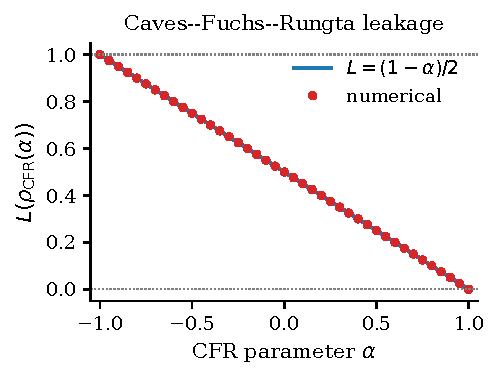
\includegraphics[width=0.55\linewidth]{../figures/fig_cfr.pdf}
\caption{Leakage of the Caves--Fuchs--Rungta family $\rho_{\mathrm{CFR}}(\alpha)$
as a function of $\alpha$. The closed-form prediction $\Lleak=(1-\alpha)/2$ from
Proposition~\ref{prop:cfr} (solid curve) matches numerical evaluation of
$\Lleak=\Tr(\Pminus\rho_{\mathrm{CFR}}(\alpha))$ (points). At $\alpha=1$ (max
real-entangled, complex-separable) leakage vanishes; at $\alpha=-1$ (anti-aligned)
leakage equals~$1$.}
\label{fig:cfr}
\end{figure}

%%----------------------------------------------------------------------
\section{Same-$i$ leakage as a resource}
\label{sec:resource}

\subsection{Definition and basic properties}

The \textbf{same-$i$ leakage} of a real density operator $\rho$ on $\KAB$ is
\begin{equation}
  \Lleak(\rho) := \Tr(\Pminus\rho) = \tfrac{1}{2}\bigl(1+\Tr(\Mop\rho)\bigr).
  \label{eq:leakage-def}
\end{equation}
The \textbf{free face} is $\FAB=\{\rho : \Lleak(\rho)=0\}$. Manifestly $\Lleak$ is
affine in $\rho$ and bounded: $0\le\Lleak\le 1$, with $\Lleak=0$ if and only if
$\rho=\Pplus\rho\Pplus$ --- that is, $\rho$ is supported entirely in the aligned
sector. (The non-trivial direction uses $\Tr(\Pminus\rho\Pminus)=0$ together with
$\Pminus\rho\Pminus\succeq 0$, forcing $\Pminus\rho\Pminus=0$; then $\rho\succeq 0$
on the bipartite block decomposition forces the off-diagonal blocks $\rho_{+-}=0$
by Schur complement.)

The leakage $\Lleak(\rho)$ measures the probability weight outside the aligned sector
--- the chance that a sector-parity measurement returns the anti-aligned outcome. It
is insensitive to coherence between sectors. That coherence is captured separately by
the \textbf{coherent leakage}
\begin{equation}
  C(\rho) := \|\Pplus\rho\Pminus\|_1,
\end{equation}
which is the operationally relevant quantity for the discrimination task in
Section~\ref{sec:discrimination}, and which is constrained by $\Lleak$ through the
bound below.

\begin{theorem}[Coherent leakage bound]
\label{thm:coherent}
For every real density operator $\rho$,
\begin{equation}
  \|\Pplus\rho\Pminus\|_1 \;\le\; \sqrt{\Lleak(\rho)\bigl(1-\Lleak(\rho)\bigr)},
  \label{eq:coherent-bound}
\end{equation}
with equality on pure coherent cross-sector states.
\end{theorem}

\emph{Proof sketch.} Douglas factorization for PSD block matrices~\cite{Bhatia1997}
writes $\rho_{+-}=\rho_{++}^{1/2}K\rho_{--}^{1/2}$ with $\|K\|_\infty\le 1$;
H\"older then gives $\|\rho_{+-}\|_1\le\sqrt{\Tr\rho_{++}}\sqrt{\Tr\rho_{--}}
=\sqrt{(1-\Lleak)\Lleak}$. Saturation by
$|\psi\rangle=\sqrt{1-\lambda}|\psi_+\rangle+\sqrt{\lambda}|\psi_-\rangle$ is
direct. See Appendix~\ref{app:proofs} for details. \hfill$\square$

\begin{figure}[htbp]
\centering
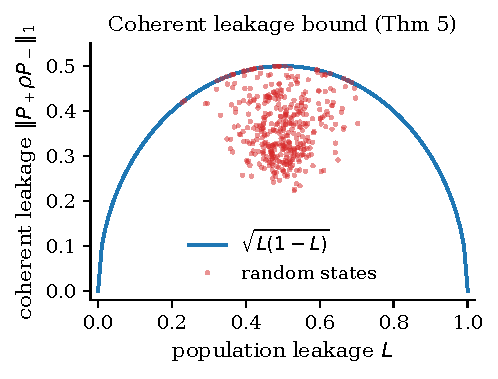
\includegraphics[width=0.6\linewidth]{../figures/fig_coherent_bound.pdf}
\caption{Coherent leakage $\|\Pplus\rho\Pminus\|_1$ against population leakage
$\Lleak(\rho)$. Solid curve: saturation envelope $\sqrt{\Lleak(1-\Lleak)}$ from
Theorem~\ref{thm:coherent}. Red dots: $400$ random real density operators of varying
rank on $\KAB$ with $d_A=d_B=2$. Black stars: pure coherent cross-sector states,
which saturate the bound. Orange squares: block-diagonal states, which lie on the
$C=0$ axis regardless of $\Lleak$.}
\label{fig:coherent}
\end{figure}

\subsection{Free operations}

\begin{theorem}[Leakage monotonicity criterion]
\label{thm:monotonicity}
A real CPTP map $\Phi$ on $\KAB$ satisfies $\Lleak(\Phi(\rho))\le\Lleak(\rho)$ for
every density operator $\rho$ iff $\Phid(\Pminus)\le\Pminus$.
\end{theorem}

(Forward direction by duality: $\Lleak(\Phi(\rho))-\Lleak(\rho)=
\Tr((\Phid(\Pminus)-\Pminus)\rho)$. Full proof in Appendix~\ref{app:proofs}.)

\begin{theorem}[Kraus criterion for leakage-nonincreasing channels]
\label{thm:kraus}
For a real CP map $\Phi(\rho)=\sum_k K_k\rho K_k^\top$ satisfying
$\sum_k K_k^\top K_k=I$, the condition $\Phid(\Pminus)\le\Pminus$ holds iff
\begin{equation}
  \Pminus K_k\Pplus = 0 \qquad\text{for every }k.
\end{equation}
\end{theorem}

(Proof in Appendix~\ref{app:proofs}.)

\begin{definition}[Strongly sector-preserving channels]
\label{def:sector-preserving}
A real CPTP channel $\Phi$ with Kraus operators $\{K_k\}$ is \emph{strongly
sector-preserving} if $[K_k,\Mop]=0$ for every $k$. Strongly sector-preserving
channels conserve leakage exactly: $\Lleak(\Phi(\rho))=\Lleak(\rho)$.
\end{definition}

%%----------------------------------------------------------------------
\section{Geometry of the resource}
\label{sec:geometry}

\subsection{Trace distance to the free face on coherent pure states}

\begin{theorem}[Trace distance to the free face: coherent pure states]
\label{thm:tracedist}
Let $|\psi\rangle=\sqrt{1-\lambda}|\psi_+\rangle+\sqrt{\lambda}|\psi_-\rangle$ with
$|\psi_\pm\rangle\in H_\pm$ unit and $0\le\lambda\le 1$. Then
\begin{equation}
  D_1\bigl(|\psi\rangle\langle\psi|,\FAB\bigr)
  := \inf_{\sigma\in\FAB}\tfrac{1}{2}\bigl\||\psi\rangle\langle\psi|-\sigma\bigr\|_1
  = \sqrt{\lambda}.
\end{equation}
\end{theorem}

\emph{Proof sketch.} Upper bound: $\sigma=|\psi_+\rangle\langle\psi_+|\in\FAB$ gives
$\tfrac{1}{2}\||\psi\rangle\langle\psi|-\sigma\|_1
=\sqrt{1-|\langle\psi|\psi_+\rangle|^2}=\sqrt{\lambda}$. The matching lower bound is
achieved via an explicit dual witness $Y$ on $\operatorname{span}\{\psi_+,\psi_-\}$;
see Appendix~\ref{app:proofs}. \hfill$\square$

\subsection{Alignment weight}

The convex-roof alignment weight is
\begin{equation}
  W(\rho) := \inf\{\lambda\in[0,1] :
  \rho=(1-\lambda)\sigma+\lambda\tau,\;\sigma\in\FAB,\;\tau\in\mathcal{D}(\KAB)\}.
\end{equation}

\begin{proposition}[Alignment weight ordering]
\label{prop:weight}
$W(\rho)\ge\Lleak(\rho)$, with equality on states block-diagonal in $\Hplus\oplus\Hminus$.
For coherent pure cross-sector states with $0<\lambda<1$, $W=1$ while
$\Lleak=\lambda$.
\end{proposition}

\begin{proof}
If $\rho=(1-\lambda)\sigma+\lambda\tau$ with $\sigma$ free, then
$\Lleak(\rho)=\lambda\Lleak(\tau)\le\lambda$; taking the infimum gives $\Lleak\le W$.
For block-diagonal $\rho$, the decomposition $\rho=(\rho_{++}\oplus 0)+(0\oplus\rho_{--})$
realizes $W=\Lleak$. For a coherent pure state, extremality forces the decomposition
to be trivial ($\sigma=|\psi\rangle\langle\psi|$ is not free), so $W=1$.
\end{proof}

\subsection{Divergent positive-noise generalized robustness}

\begin{proposition}[Divergent positive-noise generalized robustness]
\label{prop:robustness}
The standard generalized robustness
\begin{equation}
  R(\rho) := \inf\{s\ge 0 : (\rho+s\tau)/(1+s)\in\FAB,\;\tau\in\mathcal{D}(\KAB)\}
\end{equation}
is infinite whenever $\Lleak(\rho)>0$.
\end{proposition}

\begin{proof}
If $(\rho+s\tau)/(1+s)\in\FAB$, then $\Pminus(\rho+s\tau)\Pminus=0$. Both
$\Pminus\rho\Pminus$ and $\Pminus\tau\Pminus$ are PSD, and their sum vanishes only if
each vanishes. Hence $\Lleak(\rho)=0$.
\end{proof}

The divergence is structural: it reflects that $\FAB$ is a proper face of the state
space (not an interior region of a convex cone of ``noisy free states''), and is
therefore generic for sector-grading resource theories. It also means that the
standard Takagi--Regula~\cite{TakagiRegula2019} robustness-quantifies-advantage
framework does not directly apply; the operational quantifier in our setting is trace
distance, not robustness.

\subsection{Object summary}
\label{sec:object-summary}

\begin{center}
\renewcommand{\arraystretch}{1.15}
\begin{tabular}{@{}lll@{}}
\toprule
Object & Formula & Physical meaning \\
\midrule
$J_A,J_B$ & $J^2=-I,\;J^\top=-J$ & Local complex structures \\
$\Mop$ & $J_A\otimes J_B$ & Alignment operator \\
$H_\pm$ & $\ker(\Mop\pm I)$ & Aligned / anti-aligned sectors \\
$P_\pm$ & $\tfrac{1}{2}(I\mp\Mop)$ & Sector projectors \\
$\Lleak(\rho)$ & $\Tr(\Pminus\rho)$ & Population leakage \\
$C(\rho)$ & $\|\Pplus\rho\Pminus\|_1$ & Coherent leakage \\
$W(\rho)$ & convex-roof alignment weight & Mixture resource \\
$D_1(\rho,\FAB)$ & $\inf_{\sigma\in\FAB}\tfrac{1}{2}\|\rho-\sigma\|_1$
  & Trace distance to free face \\
$R(\rho)$ & generalized robustness & $=\infty$ for $\Lleak>0$ \\
\bottomrule
\end{tabular}
\end{center}

%%----------------------------------------------------------------------
\section{Dynamics}
\label{sec:dynamics}

Up to this point the framework has been static. We now ask: what dynamics preserve,
generate, or destroy same-$i$ leakage? A Hamiltonian generator $G$ that commutes
with $\Mop$ produces leakage-conserving evolution; perturbations breaking that
commutation generate leakage at quadratic order in the perturbation strength; and
dissipative Lindblad evolutions admit an explicit rate formula whose vanishing is
characterised by a simple commutator condition on the jump operators. These results
convert the abstract sector structure into a usable physical predictor: given a
real-Hilbert-space model with explicit dynamics, one can check whether leakage is
conserved by inspection.

\subsection{Hamiltonian leakage}

Let $H_\R$ be a real symmetric Hamiltonian on $\KAB$. The Schr\"{o}dinger generator
is $G=-JH_\R$, which is skew-symmetric ($G^\top=-G$), so the evolution $O(t)=e^{Gt}$
is orthogonal.

\begin{theorem}[Hamiltonian leakage conservation]
\label{thm:hamiltonian}
If $[G,\Mop]=0$, then $\Lleak(\rho(t))=\Lleak(\rho(0))$ for all $t$.
\end{theorem}

\begin{proof}
$[G,\Mop]=0$ implies $[e^{Gt},\Pminus]=0$, so
$\Tr(\Pminus e^{Gt}\rho e^{-Gt})=\Tr(\Pminus\rho)$.
\end{proof}

\subsection{Perturbative leakage generation}

\begin{theorem}[Perturbative leakage]
\label{thm:perturbative}
Let $G_\epsilon=G_0+\epsilon B$ with $G_0^\top=-G_0$, $B^\top=-B$, and
$[G_0,\Mop]=0$. For $\psi_0\in\Hplus$ unit and finite $t>0$,
\begin{equation}
  \Lleak\bigl(|e^{G_\epsilon t}\psi_0\rangle\langle e^{G_\epsilon t}\psi_0|\bigr)
  = \epsilon^2\left\|\int_0^t\Pminus e^{G_0(t-s)}Be^{G_0 s}\psi_0\,ds\right\|^2
  + O(\epsilon^3).
\end{equation}
\end{theorem}

(Duhamel-expansion proof in Appendix~\ref{app:proofs}.)

\subsection{Lindblad leakage rate}

A real Lindblad generator and its dual are
\begin{equation}
  \mathcal{L}(\rho) = G\rho+\rho G^\top
  +\sum_\ell\bigl(R_\ell\rho R_\ell^\top-\tfrac{1}{2}\{R_\ell^\top R_\ell,\rho\}\bigr),
  \quad
  \Ldag(X) = [X,G]+\sum_\ell\bigl(R_\ell^\top XR_\ell
  -\tfrac{1}{2}\{R_\ell^\top R_\ell,X\}\bigr).
  \label{eq:lindblad}
\end{equation}

\begin{theorem}[Lindblad leakage rate]
\label{thm:lindblad}
$\dfrac{d}{dt}\Lleak(\rho_t) = \Tr\bigl(\Ldag(\Pminus)\rho_t\bigr)$. If
$\Ldag(\Pminus)=0$, leakage is conserved; if $\Ldag(\Pminus)\le 0$, leakage is
nonincreasing.
\end{theorem}

\begin{corollary}[Sufficient conservation condition]
\label{cor:lindblad}
If $[G,\Mop]=0$ and $[R_\ell,\Mop]=0$ for every $\ell$, then $\Ldag(\Pminus)=0$
and $\Lleak(\rho_t)=\Lleak(\rho_0)$ for all $t$.
\end{corollary}

\begin{proof}
$[G,\Mop]=0$ implies $[\Pminus,G]=0$, so the Hamiltonian-commutator term in
$\Ldag(\Pminus)$ vanishes. For each dissipator, $[R_\ell,\Mop]=0$ gives
$[R_\ell,\Pminus]=0$ and $[R_\ell^\top,\Pminus]=0$, hence
$R_\ell^\top R_\ell$ commutes with $\Pminus$. Then
$R_\ell^\top\Pminus R_\ell=R_\ell^\top R_\ell\Pminus
=\tfrac{1}{2}\{R_\ell^\top R_\ell,\Pminus\}$, so each dissipator term vanishes.
\end{proof}

%%----------------------------------------------------------------------
\section{Sector-parity discrimination}
\label{sec:discrimination}

So far the framework has been structural and dynamical; we now extract an operational
task. Suppose a verifier hands Alice a black-box channel that is either the identity
$\mathcal{N}_0(\rho)=\rho$ or the sector-parity flip $\mathcal{N}_1(\rho)=\Mop\rho\Mop$,
with equal prior. Alice prepares a probe state $\rho$ whose leakage is bounded by
$\epsilon$, sends it through the box, and measures the output. What is her optimal
probability of correctly identifying the channel?

This task is not a network witness --- there is no spatial separation involved, no
source-independence requirement, and the channel $\Mop\rho\Mop$ is constructed by
hand rather than emerging from a physical scenario. Rather, it is the simplest
internal operational probe of the resource theory: a ``minimum-effort'' task whose
closed-form optimum demonstrates how leakage and coherent cross-sector amplitude
translate into distinguishability. The optimal strategy involves coherent cross-sector
probes; pure population leakage is operationally inert.

\begin{theorem}[Sector-parity discrimination]
\label{thm:discrimination}
The optimal binary discrimination success probability with equal priors and leakage
budget $\Lleak(\rho)\le\epsilon$ is
\begin{equation}
  p_{\mathrm{succ}}^{(\epsilon)} = \tfrac{1}{2}+\sqrt{m(1-m)},\qquad
  m=\min\{\epsilon,1/2\}.
\end{equation}
Equivalently, $p_{\mathrm{succ}}^{(\epsilon)}=\tfrac{1}{2}+\sqrt{\epsilon(1-\epsilon)}$
for $0\le\epsilon\le 1/2$, and $p_{\mathrm{succ}}^{(\epsilon)}=1$ for
$\epsilon\ge 1/2$, saturated by coherent pure cross-sector states.
\end{theorem}

\begin{proof}
The matrix $X:=\Pplus\rho\Pminus+\Pminus\rho\Pplus$ has off-diagonal block structure
with $B=\Pplus\rho\Pminus$; its eigenvalues come in pairs $\pm\sigma_i(B)$, so
$\|X\|_1=2\|B\|_1$. Hence $\|\rho-\Mop\rho\Mop\|_1=4\|\Pplus\rho\Pminus\|_1$,
and the Holevo--Helstrom theorem~\cite{Helstrom1976} gives
$p_{\mathrm{succ}}(\rho)=\tfrac{1}{2}+\|\Pplus\rho\Pminus\|_1$. Maximising over
$\{\rho:\Lleak(\rho)\le\epsilon\}$ using Theorem~\ref{thm:coherent}: the function
$\Lleak\mapsto\sqrt{\Lleak(1-\Lleak)}$ is increasing on $[0,1/2]$ and peaks at
$\Lleak=1/2$. For $\epsilon<1/2$ the constraint is tight and the optimum is at
$\Lleak=\epsilon$; for $\epsilon\ge 1/2$ the unconstrained optimum $\Lleak=1/2$
satisfies the budget. The bound is saturated by the pure coherent cross-sector state
$|\psi\rangle=\sqrt{1-m}|\psi_+\rangle+\sqrt{m}|\psi_-\rangle$ with
$m=\min\{\epsilon,1/2\}$.
\end{proof}

\paragraph{Block-diagonal probes give no advantage.} For $\rho$ block-diagonal on
$\Hplus\oplus\Hminus$, $\Pplus\rho\Pminus=0$ and $p_{\mathrm{succ}}(\rho)=1/2$.
Population leakage alone provides no advantage; only coherent cross-sector amplitude
does.

\paragraph{Limitation: imaginarity is not separated by this task.} The optimal probe
can be chosen with entrywise-real entries in the basis where $J_A,J_B$ are the
standard symplectic matrices: take $\psi_+,\psi_-\in H_\pm$ unit and entrywise real
(always possible since $H_\pm$ are real subspaces); then $|\psi\rangle\langle\psi|$
is entrywise real and has Hickey--Gour imaginarity zero in that basis, yet it achieves
the maximal success probability.

\begin{figure}[htbp]
\centering
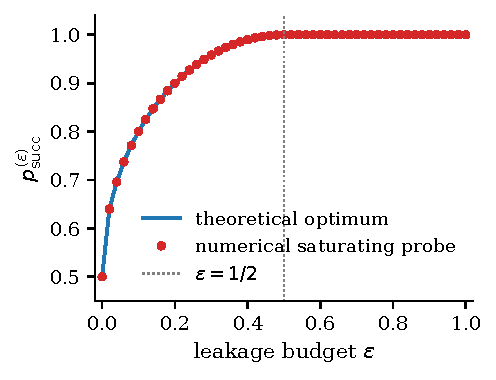
\includegraphics[width=0.55\linewidth]{../figures/fig_discrimination.pdf}
\caption{Sector-parity optimal success probability as a function of leakage budget
$\epsilon$. Solid curve: theoretical optimum $\tfrac{1}{2}+\sqrt{m(1-m)}$,
$m=\min\{\epsilon,1/2\}$. Points: numerical saturating probe. The vertical line at
$\epsilon=1/2$ marks where the optimum reaches $1$.}
\label{fig:discrimination}
\end{figure}

%%----------------------------------------------------------------------
\section{Structural distinction from basis imaginarity}
\label{sec:imaginarity}

The Hickey--Gour resource theory of imaginarity~\cite{HickeyGour2018,Wu2021Imaginarity}
defines a state as ``free'' if its density matrix has only real entries in a fixed
reference basis. This is a \emph{basis-relative} notion. Same-$i$ leakage, by
contrast, depends only on the local complex structures $J_A,J_B$ and is
basis-independent. The two are therefore distinct resources, but the precise nature
of the distinction is example-based, not operational. We illustrate this with two
extremal cases. \AA berg~\cite{Aberg2006} introduced the closely related superposition
quantification framework that motivates both notions.

\begin{example}[Entrywise real, $\Lleak=1/2$]
\label{ex:realL}
Let $\psi_\pm\in H_\pm$ be entrywise-real unit vectors (possible because $H_\pm$ are
real subspaces). Take $\psi=(\psi_++\psi_-)/\sqrt{2}$. Then
$\rho=|\psi\rangle\langle\psi|$ has entirely real entries in the standard basis ---
so its Hickey--Gour imaginarity is zero in that basis --- but $\Lleak(\rho)=1/2$.
\end{example}

\begin{example}[$\Lleak=0$, nonzero entrywise imaginarity]
\label{ex:complexL0}
Let $|\psi\rangle_\C=(|00\rangle+i|11\rangle)/\sqrt{2}$ on $\C^2\otimes_\C\C^2$.
Its density operator has nonzero imaginary entries in the computational basis. Apply
$\iota$ from Eq.~\eqref{eq:iota}: $\iota(|\psi\rangle_\C)$ is a unit vector in
$\Hplus\subset\KAB$, and $\rho_R=|\iota(|\psi\rangle_\C)\rangle\langle\iota(|\psi\rangle_\C)|$
satisfies $\Lleak(\rho_R)=0$ by construction.
\end{example}

Examples~\ref{ex:realL} and~\ref{ex:complexL0} demonstrate that no map
$\Lleak\mapsto\mathcal{I}_B$ and no map $\mathcal{I}_B\mapsto\Lleak$ exists that is
consistent across the standard real basis: the two measures are structurally distinct.
Whether there exists an operational task --- a channel pair and probe class --- for
which $\Lleak$-advantage cannot be achieved by any zero-imaginarity state in any basis
is open. We conjecture that no such task exists for two-rebit channels, and that the
simplest separating task requires composition of $d_A=d_B=2$ systems with
non-trivial entanglement structure; this is a natural follow-up direction.

%%----------------------------------------------------------------------
\section{The Caves--Fuchs--Rungta family revisited}
\label{sec:cfr-revisit}

We computed in Section~\ref{sec:cfr} that $\Lleak(\rho_{\mathrm{CFR}}(\alpha))=(1-\alpha)/2$.
We extract two further geometric statements that this family makes vivid.

\paragraph{Position in the coherent-leakage diagram.} Since
$\rho_{\mathrm{CFR}}(\alpha)=\tfrac{1}{4}(I-\alpha\Mop)$ is block-diagonal in
$\Hplus\oplus\Hminus$ (both the identity and $\Mop$ are block-diagonal in this
decomposition), its coherent leakage $C(\rho_{\mathrm{CFR}}(\alpha))=0$ for all
$\alpha$. The CFR family therefore lies on the $C=0$ axis of Figure~\ref{fig:coherent},
regardless of $\alpha$.

\paragraph{Perturbative dynamics.} Applying the perturbative leakage formula
(Theorem~\ref{thm:perturbative}) to an initial CFR state $\rho_0=\rho_{\mathrm{CFR}}(1)
=\tfrac{1}{2}\Pplus$ under a perturbation that breaks $[G_0,\Mop]=0$: since
$\rho_0$ is supported in $\Hplus$, any first-order Duhamel contribution is killed by
$\Pminus$, and leakage grows as $O(\epsilon^2)$, consistent with the block-diagonal
structure.

\paragraph{Connection to the ubit construction.} Aleksandrova--Borish--Wootters~%
\cite{AleksandrovaBorishWootters2013} couple a real system to an auxiliary rebit
(``ubit'') to recover complex predictions. The CFR two-rebit state at $\alpha=1$
corresponds to maximal alignment between Alice's and Bob's $i$-structures, which is
precisely the condition the ubit construction enforces by hand. Same-$i$ leakage
quantifies how far a general state deviates from that enforced alignment.

%%----------------------------------------------------------------------
\section{A structural obstruction to product-source bilocal witnesses}
\label{sec:bobnode}

Same-$i$ leakage is a property of an actual real-Hilbert-space state. To turn it into
a network witness --- a statement that some experimentally observable correlation
cannot be reproduced by any real-source bilocal model --- one would naively define a
Bob-node leakage parameter $\Lleak_B$ on the reduced state $\rho_{B_1B_2}$ and look
for sources with $\Lleak_B>1/2$. We now show that this naive programme fails for a
structural reason: for every \emph{product} bilocal source
$\rho_{B_1B_2}=\rho_{B_1}\otimes\rho_{B_2}$, the Bob-node leakage is identically
$1/2$. This is not a contingent failure; it is a no-go theorem with a one-line proof.

Consider the bilocal scenario $A\leftarrow S_1\to B\leftarrow S_2\to C$, with
independent product sources $\rho_{\mathrm{net}}=\rho_{AB_1}\otimes_\R\rho_{B_2C}$.
The natural Bob-node alignment operator is $\Mop_B=J_{B_1}\otimes J_{B_2}$, and
$\Lleak_B(\rho_{B_1B_2}):=\Tr(\Pminus^B\rho_{B_1B_2})$ with
$\Pminus^B=\tfrac{1}{2}(I+\Mop_B)$.

\begin{proposition}[Bob-node obstruction]
\label{prop:bobnode}
For every product bilocal source $\rho_{B_1B_2}=\rho_{B_1}\otimes_\R\rho_{B_2}$
with $\rho_{B_i}$ real symmetric PSD,
\begin{equation}
  \Lleak_B(\rho_{B_1B_2}) = \tfrac{1}{2}\quad\text{exactly.}
\end{equation}
\end{proposition}

\begin{proof}
$\Tr(\Mop_B\,\rho_{B_1}\otimes\rho_{B_2})=\Tr(J_{B_1}\rho_{B_1})\cdot\Tr(J_{B_2}\rho_{B_2})$.
Real symmetric $\rho$ and real antisymmetric $J$ satisfy
$\Tr(J\rho)=\Tr((J\rho)^\top)=\Tr(\rho^\top J^\top)=-\Tr(J\rho)$,
hence $\Tr(J\rho)=0$. Each factor vanishes, so
$\Lleak_B=\tfrac{1}{2}(1+0)=\tfrac{1}{2}$.
\end{proof}

The obstruction has two consequences, one negative and one positive.
\textbf{Negative:} no quantity built linearly from the marginal $\rho_{B_1B_2}$
in a product bilocal model can detect alignment, because the linear functional
$\Tr(\Mop_B\,\cdot)$ vanishes identically. Network certification of same-$i$ leakage
cannot proceed via the most direct route.
\textbf{Positive:} the obstruction identifies precisely which feature of the bilocal
scenario must be relaxed for a non-trivial witness to exist. Three natural
alternatives are: (i)~replacing product-state with operational source independence
in the sense of Hoffreumon--Woods~\cite{HoffreumonWoods2025,HoffreumonWoodsNonFalsified};
(ii)~constructing the witness from a non-product correlation functional involving
Alice's and Charlie's measurement settings that survives the Bob-node marginalisation;
(iii)~restricting to $J$-covariant sources, in which case the algebraic identity
producing $1/2$ no longer holds. The obstruction makes precise what work remains.

%%----------------------------------------------------------------------
\section{Discussion}
\label{sec:discussion}

\subsection{What does same-$i$ leakage teach us about real vs.\ complex composition?}

Ordinary complex composition is exactly the zero-leakage, aligned sector of a
strictly larger real tensor product. Real Hilbert space accommodates more than
complex Hilbert space in bipartite systems, and the ``more'' is a well-defined
resource with affine monotone, exactly characterised free operations, and operational
meaning via the sector-parity discrimination task. The divergence of the standard
positive-noise robustness (Proposition~\ref{prop:robustness}) reflects that the free
face is a proper face, not a symmetry orbit, of the state space.

\subsection{Why is same-$i$ leakage not just imaginarity?}

Imaginarity is basis-relative; same-$i$ leakage is basis-independent. Examples~%
\ref{ex:realL} and~\ref{ex:complexL0} establish structural inequivalence. Operational
separation remains open and is conjectured to require $d_A=d_B=2$ systems with
non-trivial entanglement structure. The sector-parity discrimination task can be
saturated by entrywise-real probes (Section~\ref{sec:discrimination}), so it does
not operationally separate the two resources.

\subsection{Why do product-source bilocal network witnesses fail?}

Proposition~\ref{prop:bobnode} is the structural answer: the linear functional
$\Tr(\Mop_B\,\cdot)$ vanishes identically on product real density operators.
Three alternative routes exist --- operational independence, non-product correlation
functionals, $J$-covariant sources --- each open.

\subsection{What is still missing for a stronger foundations claim?}

A non-tautological device-independent network certificate that uses operational
rather than product-state source independence, plus its connection to the
Hoffreumon--Woods~\cite{HoffreumonWoods2025,HoffreumonWoodsNonFalsified} and
Weilenmann--Gisin--Sekatski~\cite{WeilenmannGisinSekatski2025} lines of work. The
framework extends to $N$ parties via the multiparty alignment projector
$P_{\mathrm{phys}}=\prod_{i=2}^N\tfrac{1}{2}(I-\Aop_1\Aop_i)$; the multiparty
monotone, its dynamics, and its operational tasks are open. Asymptotic conversion
rates between coherent and population leakage, and distillation under free
operations, are also open.

%%----------------------------------------------------------------------
\section{Reproducibility}
\label{sec:reproducibility}

A companion code repository implements the constructions of this paper as a Python
package and includes a pytest suite of $59$ numerical sanity checks. These checks
confirm the algebraic identities of Section~\ref{sec:samei} (sector projectors, the
embedding $\iota$, the alignment trace identity), the inequality of
Theorem~\ref{thm:coherent} on random PSD states ($4$-, $8$-, and $16$-dimensional,
$10^4$ trials each), the perturbative scaling of Theorem~\ref{thm:perturbative}, the
conservation condition of Corollary~\ref{cor:lindblad}, the closed-form CFR leakage
of Proposition~\ref{prop:cfr}, the Bob-node obstruction of Proposition~%
\ref{prop:bobnode} on product sources, and the discrimination optimum of
Theorem~\ref{thm:discrimination}. Tolerances are $10^{-10}$ for algebraic identities
and $10^{-3}$ for Euler-integrated Lindblad dynamics. All figures are generated by
\texttt{figures/make\_figures.py}.

The repository is distributed under the MIT License at
\url{https://github.com/JulianAttemptsCoding/complex_quantum_compute_theory}.
We do not claim the code verifies theorems; the code checks that the theorems'
predictions match numerical computation on specific examples.

\bibliographystyle{quantum}
\bibliography{refs}

%%======================================================================
\appendix

\section{Theorem inventory}
\label{app:inventory}

\begin{center}
\renewcommand{\arraystretch}{1.25}
\begin{tabular}{@{}lll@{}}
\toprule
Label & Statement & Location \\
\midrule
Theorem~\ref{thm:realification}
  & Realification preserves statistics, $\rho_\R=\tfrac{1}{2}R(\rho_\C)$.
  & \S\ref{sec:realification}, proof App.~\ref{app:proofs} \\
Theorem~\ref{thm:quotient}
  & Same-$i$ quotient: $(\HC^A\otimes_\C\HC^B)_\R\cong\KAB/\operatorname{span}\{J_Ax\otimes y-x\otimes J_By\}$.
  & \S\ref{sec:samei} \\
Theorem~\ref{thm:sector}
  & Aligned sector $\Hplus=\ker(\Mop+I)$ carries induced complex structure $\JAB$.
  & \S\ref{ssec:sector} \\
Proposition~\ref{prop:cfr}
  & CFR leakage $\Lleak(\rho_{\mathrm{CFR}}(\alpha))=(1-\alpha)/2$.
  & \S\ref{sec:cfr} \\
Def.~\ref{def:sector-preserving}
  & Same-$i$ leakage $\Lleak(\rho):=\Tr(\Pminus\rho)$; free face $\FAB$.
  & \S\ref{sec:resource} \\
Theorem~\ref{thm:coherent}
  & Coherent leakage bound $\|\Pplus\rho\Pminus\|_1\le\sqrt{\Lleak(1-\Lleak)}$.
  & \S\ref{sec:resource}, proof App.~\ref{app:proofs} \\
Theorem~\ref{thm:monotonicity}
  & Monotonicity iff $\Phid(\Pminus)\le\Pminus$.
  & \S\ref{sec:resource}, proof App.~\ref{app:proofs} \\
Theorem~\ref{thm:kraus}
  & Kraus criterion for leakage-nonincreasing: $\Pminus K_k\Pplus=0$.
  & \S\ref{sec:resource}, proof App.~\ref{app:proofs} \\
Theorem~\ref{thm:tracedist}
  & $D_1(|\psi\rangle\langle\psi|,\FAB)=\sqrt{\lambda}$ on coherent pure states.
  & \S\ref{sec:geometry}, proof App.~\ref{app:proofs} \\
Proposition~\ref{prop:weight}
  & $W\ge\Lleak$; $W=\Lleak$ block-diagonally; $W=1$ on coherent pure.
  & \S\ref{sec:geometry} \\
Proposition~\ref{prop:robustness}
  & Divergent positive-noise generalized robustness: $R=\infty$ when $\Lleak>0$.
  & \S\ref{sec:geometry} \\
Theorem~\ref{thm:hamiltonian}
  & Hamiltonian leakage conservation when $[G,\Mop]=0$.
  & \S\ref{sec:dynamics} \\
Theorem~\ref{thm:perturbative}
  & Perturbative leakage $O(\epsilon^2)$.
  & \S\ref{sec:dynamics}, proof App.~\ref{app:proofs} \\
Theorem~\ref{thm:lindblad}
  & Lindblad rate $\dot\Lleak=\Tr(\Ldag(\Pminus)\rho_t)$.
  & \S\ref{sec:dynamics} \\
Corollary~\ref{cor:lindblad}
  & $[G,\Mop]=0=[R_\ell,\Mop]$ for all $\ell$ implies exact Lindblad conservation.
  & \S\ref{sec:dynamics} \\
Theorem~\ref{thm:discrimination}
  & Sector-parity discrimination optimum $\tfrac{1}{2}+\sqrt{m(1-m)}$.
  & \S\ref{sec:discrimination} \\
Proposition~\ref{prop:bobnode}
  & Bob-node obstruction $\Lleak_B=1/2$ for product bilocal sources.
  & \S\ref{sec:bobnode} \\
Theorem~\ref{thm:moments}
  & Moment-matrix soundness (SDP oracle).
  & App.~\ref{app:sdp} \\
\bottomrule
\end{tabular}
\end{center}

%%----------------------------------------------------------------------
\section{Proofs of main results}
\label{app:proofs}

\subsection*{Proof of Theorem~\ref{thm:realification}}

The map $R$ is a unital ring homomorphism: $R(XY)=R(X)R(Y)$ by direct block
computation. For $X=A+iB$, $\Tr_\R R(X)=2\Tr A=2\Re\Tr_\C X$. Since $\rho_\C$ is
Hermitian, $\Tr\rho_\C\in\R$ and equals $1$, so $\Tr_\R R(\rho_\C)=2$, giving
$\Tr_\R\rho_\R=1$. Therefore
\[
  \Tr_\R(E_\R\rho_\R) = \tfrac{1}{2}\Tr_\R R(E_\C\rho_\C)
  = \Re\Tr_\C(E_\C\rho_\C) = \Tr_\C(E_\C\rho_\C),
\]
where the last equality uses that the trace of a product of Hermitian operators is
real. \hfill$\square$

\subsection*{Proof of Theorem~\ref{thm:coherent} (Coherent leakage bound)}

By the Douglas factorization for PSD block matrices~\cite{Bhatia1997}, there exists a
contraction $K$ with $\|K\|_\infty\le 1$ such that $\rho_{+-}=\rho_{++}^{1/2}K\rho_{--}^{1/2}$.
By the multiplicative trace-norm bound,
\[
  \|\rho_{+-}\|_1 \le \|\rho_{++}^{1/2}\|_2\|K\|_\infty\|\rho_{--}^{1/2}\|_2
  \le \sqrt{\Tr\rho_{++}}\sqrt{\Tr\rho_{--}} = \sqrt{(1-\Lleak)\Lleak}.
\]
For the pure state $|\psi\rangle=\sqrt{1-\lambda}|\psi_+\rangle+\sqrt{\lambda}|\psi_-\rangle$
with $|\psi_\pm\rangle\in H_\pm$ unit, direct computation gives $\Lleak=\lambda$ and
$\|\Pplus|\psi\rangle\langle\psi|\Pminus\|_1=\sqrt{\lambda(1-\lambda)}$. \hfill$\square$

\subsection*{Proof of Theorem~\ref{thm:monotonicity}}

$(\Leftarrow)$\; $\Lleak(\Phi(\rho))=\Tr(\Pminus\Phi(\rho))=\Tr(\Phid(\Pminus)\rho)
\le\Tr(\Pminus\rho)=\Lleak(\rho)$.

$(\Rightarrow)$\; Since $\Phi$ is real CP and $\Pminus$ is real symmetric, $\Phid(\Pminus)$
is real symmetric. The inequality $\Tr((\Phid(\Pminus)-\Pminus)\rho)\le 0$ for every
real density $\rho$ forces $\Phid(\Pminus)-\Pminus\le 0$: test on rank-one
$\rho=|v\rangle\langle v|$ for arbitrary real unit $v$. \hfill$\square$

\subsection*{Proof of Theorem~\ref{thm:kraus}}

$(\Rightarrow)$\; Compressing $\Phid(\Pminus)\le\Pminus$ to $\Hplus$:
\[
  \Pplus\Phid(\Pminus)\Pplus
  = \sum_k(\Pminus K_k\Pplus)^\top(\Pminus K_k\Pplus) \le \Pplus\Pminus\Pplus = 0.
\]
Each summand is PSD and sums to zero, so each vanishes.

$(\Leftarrow)$\; In block form $K_k=\bigl(\begin{smallmatrix}K_{++,k}&K_{+-,k}\\0&K_{--,k}\end{smallmatrix}\bigr)$,
so $K_k^\top\Pminus K_k=\bigl(\begin{smallmatrix}0&0\\0&K_{--,k}^\top K_{--,k}\end{smallmatrix}\bigr)$.
Trace preservation gives $\sum_k(K_{+-,k}^\top K_{+-,k}+K_{--,k}^\top K_{--,k})=I_-$,
hence $\sum_k K_{--,k}^\top K_{--,k}\le I_-$ and $\Phid(\Pminus)\le\Pminus$.
\hfill$\square$

\subsection*{Proof of Theorem~\ref{thm:tracedist} (lower bound)}

Let $\sigma\in\FAB$. Decompose $\sigma=\alpha|\psi_+\rangle\langle\psi_+|+(1-\alpha)\tau$
with $\alpha\in[0,1]$ and $\tau$ supported in $\Hplus\ominus\operatorname{span}\{\psi_+\}$.
Since $|\psi\rangle\langle\psi|-\alpha|\psi_+\rangle\langle\psi_+|$ is supported in
$\operatorname{span}\{\psi_+,\psi_-\}$ and $(1-\alpha)\tau$ is orthogonal to that
span,
\[
  \bigl\||\psi\rangle\langle\psi|-\sigma\bigr\|_1
  = \bigl\||\psi\rangle\langle\psi|-\alpha|\psi_+\rangle\langle\psi_+|\bigr\|_1
  + (1-\alpha).
\]
In the basis $\{\psi_+,\psi_-\}$,
\[
  |\psi\rangle\langle\psi|-\alpha|\psi_+\rangle\langle\psi_+|
  = \begin{pmatrix} 1-\lambda-\alpha & \sqrt{\lambda(1-\lambda)} \\
    \sqrt{\lambda(1-\lambda)} & \lambda \end{pmatrix},
\]
with eigenvalues $\tfrac{1-\alpha}{2}\pm\tfrac{1}{2}\sqrt{(1-\alpha)^2+4\alpha\lambda}$,
so its trace norm equals $\sqrt{(1-\alpha)^2+4\alpha\lambda}$. Therefore
$f(\alpha):=\tfrac{1}{2}\bigl[\sqrt{(1-\alpha)^2+4\alpha\lambda}+(1-\alpha)\bigr]$
is strictly decreasing on $[0,1]$ for $\lambda\in(0,1)$, minimised at $\alpha=1$
with value $\sqrt{\lambda}$. \hfill$\square$

\subsection*{Proof of Theorem~\ref{thm:perturbative}}

Duhamel expansion: $e^{G_\epsilon t}=e^{G_0 t}+\epsilon\int_0^t e^{G_0(t-s)}Be^{G_0 s}ds
+O(\epsilon^2)$. Since $[G_0,\Mop]=0$, $e^{G_0 t}\psi_0\in\Hplus$, so
$\Pminus e^{G_0 t}\psi_0=0$. Therefore
$\Pminus\psi(t)=\epsilon\int_0^t\Pminus e^{G_0(t-s)}Be^{G_0 s}\psi_0\,ds+O(\epsilon^2)$,
and $\Lleak=\|\Pminus\psi(t)\|^2=O(\epsilon^2)$. \hfill$\square$

%%----------------------------------------------------------------------
\section{SDP soundness oracle}
\label{app:sdp}

\begin{theorem}[Moment-matrix soundness]
\label{thm:moments}
Let $\mathcal{W}$ be a finite set of real polynomial words in operators
$\{E_a^x,F_b^y,G_c^z,J_A,J_B,J_C,\ldots\}$. For any realisation with real density
operator $\rho$, the matrix $\Gamma_{u,v}=\Tr(u^\top v\,\rho)$, $u,v\in\mathcal{W}$,
is positive semidefinite.
\end{theorem}

\begin{proof}
For real coefficients $c=(c_u)$,
$c^\top\Gamma c=\Tr\bigl((\sum_u c_u u)^\top(\sum_v c_v v)\rho\bigr)=\Tr(W^\top W\rho)\ge 0$
since $W^\top W\succeq 0$.
\end{proof}

This gives a sound outer-relaxation oracle for leakage-constrained polynomial
optimisation over states and effects. Convergence of the hierarchy is not claimed.
Network-bilocal independence requires inflation or scalar-extension constructions
(see Renou--Xu--Ligthart~\cite{RenouXuLigthart2026} and
Ligthart--Gachechiladze--Gross~\cite{LigthartGachechiladzeGross2023}); extending
those to carry the algebraic constraints $J_X^2=-I$, $J_X^\top=-J_X$ together with
leakage budgets is left to future work.

Figure~\ref{fig:perturbative} (below) verifies the $O(\epsilon^2)$ perturbative
scaling of Theorem~\ref{thm:perturbative} numerically.

\begin{figure}[htbp]
\centering
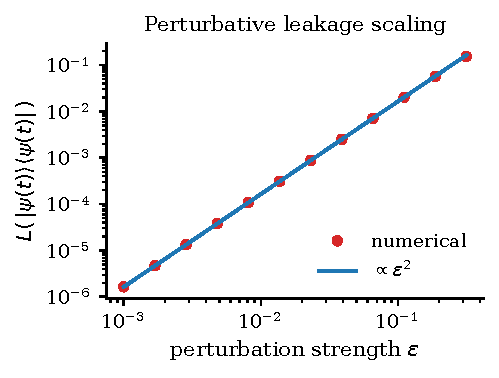
\includegraphics[width=0.55\linewidth]{../figures/fig_perturbative.pdf}
\caption{Leakage generated by a perturbation $G_0+\epsilon B$ acting on an initially
aligned ($\Lleak=0$) state, with $[G_0,\Mop]=0$. The log-log slope is $2$, confirming
the Duhamel expansion of Theorem~\ref{thm:perturbative}.}
\label{fig:perturbative}
\end{figure}

\end{document}
